\documentclass[compress,red,mathsans,10pt]{beamer}
%\documentclass[handout, compress,red,mathsans,10pt]{beamer}
\usepackage{beamerthemesplit}
\usepackage{amssymb}
%\usetheme{Antibes}
%\usepackage{pgf,pgfarrows,pgfnodes}
\usepackage[catalan]{babel}
%\usepackage[latin1]{inputenc}
\usepackage[utf8]{inputenc}
%\usepackage[pdftex]{graphicx}
\usepackage{ulem}

\setbeamercolor{uppercol}{fg=white,bg=purple}%
\setbeamercolor{lowercol}{fg=black,bg=pink}%


\usecolortheme{lily}
\begin{document}
\title{C\`alcul II}
\subtitle{Grau Telem\`atica. Curs 2012/13}  
\author{Gabriel Nicolau, Jos\'e Luis Lisani}
\date{}



\frame{\titlepage} 

%\frame{\frametitle{Table of contents}\tableofcontents} 

\section{Presentaci\'o} 
\frame{\frametitle{Informaci\'o general}	
\begin{itemize}
\item Professors: Gabriel Nicolau, Jos\'e Luis Lisani
\item [] Despatx: Anselm Turmeda D-239
\item [] E-mail: gabriel.nicolau@gmail.com, joseluis.lisani@uib.es
\item Horari:
	\begin{center}
	\begin{tabular}{|l|c|} \hline
	Dia & Hora \\ \hline
	Dimecres & 11:30 -- 13:30 \\ \hline
	Divendres & 9:30 -- 11:30 \\ \hline
	\end{tabular}
	\end{center}
\item Documentaci\'o:
	\begin{itemize}
	\item campus extens (apunts, llistes problemes, anuncis)
	\item UIB digital (guia docent, cronograma)
	\end{itemize} 
\item Tutories:
\begin{itemize}
\item Jos\'e Luis Lisani: dimarts 11h30-13h,  dijous 11h30-13h
\item Gabriel Nicolau:
\end{itemize}
\item[] <2-> \color{red}Concertau previament per email\color{black}
\end{itemize}
}


\frame{\frametitle{Temari}
\begin{itemize}
\item Tema 1. Principis de variable complexa.
	\item [] <2->\color{blue}Professor: Gabriel Nicolau. \color{red}Entrega exercicis: 22/03 \color{black}
\item Tema 2. Funcions de v\`aries variables. L\'imits i continu\"itat.
	\item [] <2->\color{blue}Professor: Jos\'e Luis Lisani. \color{red}Control: 17/04\color{black}
\item Tema 3. Funcions de v\`aries variables. Diferenciaci\'o.
	\item [] <2->\color{blue}Professor: Jos\'e Luis Lisani. \color{red}Control: 10/05 \color{black}
\item Tema 4. Funcions de v\`aries variables. Integraci\'o.
	\item [] <2->\color{blue}Professor: Gabriel Nicolau. \color{red}Entrega exercicis: 07/06  \color{black}
\item Tema 5. Introducci\'o a les equacions en derivades parcials.
	\item [] <2->\color{blue}Professor: Jos\'e Luis Lisani.\color{black}
\end{itemize}
}

\frame{\frametitle{Calendari}
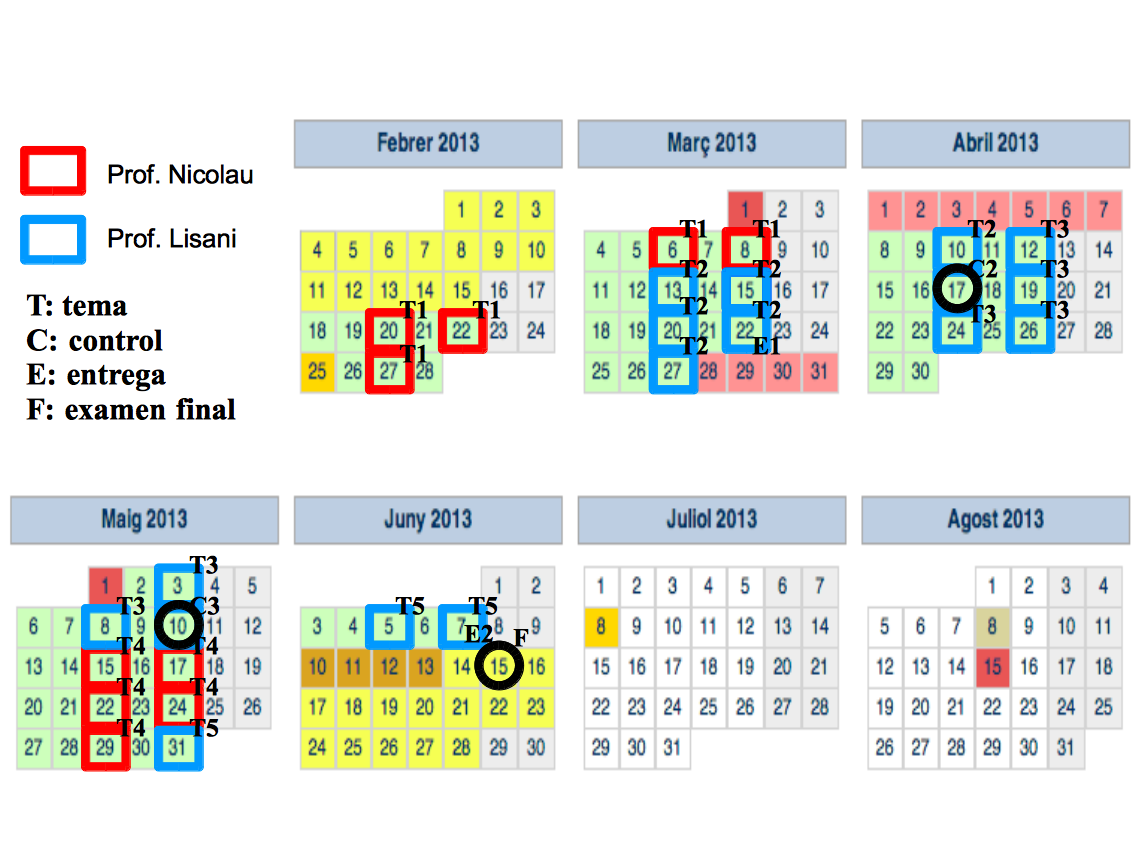
\includegraphics[width=11cm]{calendari2Sb.png}
}

\frame{\frametitle{Material}
\begin{itemize}
\item Apunts (inclouen problemes resolts) (autor: Marc Carbonell)
\item Llistes de problemes proposats (autor: Marc Carbonell)
\item Enlla\c{c}os d'inter\'es
\item[]
\item[] <2-> \color{red} Disponible a Campus Extens \color{black}
\end{itemize}
}

\frame{\frametitle{Avaluaci\'o}
\begin{itemize}
\item Activitats d'avaluaci\'o:
\begin{itemize}
\item Avaluaci\'o cont\'inua:
\begin{itemize}
\item Entrega d'exercicis: 22/03 (tema 1), 07/06 (tema 4)
\item Controls: 17/04 (tema 2), 10/05 (tema 3) 
	\item[] <2-> \color{red}Dates flexibles per a la gent que fa feina\color{black} 
\end{itemize}
\item Examen final: 15/06 (tot), \color{red}16/09 (tot)\color{black}
\end{itemize}
	\item <3-> Criteris d'avaluaci\'o:
	\begin{itemize}
	\item Nota m\'inima de l'examen final: 3
	\item Nota d'avaluaci\'o cont\'inua: 

	$70\%$ nota mitjana controls + $30\%$ nota mitjana entrega exercicis

	\item La nota de l'avaluaci\'o cont\'inua es guarda fins al setembre.
	\item Les activitats d'avaluaci\'o cont\'inua no s\'on recuperables.
	\item Nota final = $50\%$ nota avaluaci\'o continua + $50\%$ nota examen final
	\end{itemize}
\end{itemize}
}


\end{document}